% !TeX root = statnicaEKT.tex
\part{BPC-DE2 - Digitální elektronika 2}
\begin{huge}
	Otázky:
	\newline
\end{huge}
\begin{enumerate}
	\item Otázka - Reprezentace čísel pomocí signed/unsigned fixed-point, floating-point, binární, dekadická a hexadecimální soustava. 
	\item Otázka - Struktura a funkce čítačů/časovačů. Popis a využití přetečení, komparace, módy PWM. 
	\item Otázka - Sériová komunikace UART a I2C. Popis, struktura rámců a komunikačních protokolů, použití a srovnání.
	
\end{enumerate}
%%%%%%%%%%%%%%%%%%%%%%%%%%%%%%%%%%%%%%%%%%%%%%%%%%%
\chapter{Reprezentácia čísel: fixed-point, floating-point, číselné sústavy}
%%%%%%%%%%%%%%%%%%%%%%%%%%%%%%%%%%%%%%%%%%%%%%%%%%%

\section{Prečo rôzne číselné sústavy?}

Človek prirodzene používa \textbf{dekadickú sústavu} (základ 10, číslice 0--9). Digitálne obvody pracujú iba s napätiami ``nízke'' a ``vysoké'' -- prirodzene teda používajú \textbf{binárnu sústavu} (základ 2, číslice 0 a 1). \textbf{Hexadecimálna sústava} (základ 16, číslice 0--9 a a--f) slúži ako skratka pre zápis binárnych hodnôt -- jeden hex symbol zastúpi vždy presne 4 bity.

Prefixový zápis: \texttt{0b} pre binárne (napr. \texttt{0b100} = 4), \texttt{0x} pre hexadecimálne (napr. \texttt{0x1F} = 31).

\begin{center}
\begin{tabular}{ccc}
\toprule
\textbf{Dekadická} & \textbf{Binárna} & \textbf{Hexadecimálna} \\
\midrule
0  & 0000 & 0 \\
9  & 1001 & 9 \\
10 & 1010 & a \\
15 & 1111 & f \\
16 & 0001\,0000 & 10 \\
\bottomrule
\end{tabular}
\end{center}

\section{Váhovanie bitov -- ako čítať binárne číslo}

Každý bit na určitej pozícii má svoju \textbf{váhu} -- hodnotu, ktorú pridáva k celkovému číslu. Pozície sa počítajú sprava od 0, váha pozície $i$ je $2^i$.

Príklad: \texttt{1011} = $1{\cdot}8 + 0{\cdot}4 + 1{\cdot}2 + 1{\cdot}1 = 11_{10}$.

Bit s najvyššou váhou (úplne vľavo) = \textbf{MSB} (Most Significant Bit). Bit s najnižšou váhou (úplne vpravo) = \textbf{LSB} (Least Significant Bit).

Pre čísla s desatinnou časťou: bity napravo od rádovej čiarky majú záporné mocniny ($2^{-1} = 0{,}5$; $2^{-2} = 0{,}25$; atď.).

\subsection{Prevod dekadicky $\to$ binárne}

\textbf{Celá časť:} opakované delenie dvoma, zvyšky sú výsledné bity od LSB k MSB.

Príklad: $25 \div 2 = 12$ zb. \textbf{1}; $12 \div 2 = 6$ zb. \textbf{0}; $6 \div 2 = 3$ zb. \textbf{0}; $3 \div 2 = 1$ zb. \textbf{1}; $1 \div 2 = 0$ zb. \textbf{1}. Čítame zvyšky zdola nahor: $25_{10} = \texttt{11001}_2$.

\textbf{Desatinná časť:} opakované násobenie dvoma, celé časti sú výsledné bity za rádovou čiarkou.

Príklad: $0{,}375 \times 2 = \mathbf{0}{,}75$; $0{,}75 \times 2 = \mathbf{1}{,}5$; $0{,}5 \times 2 = \mathbf{1}{,}0$ $\Rightarrow$ $0{,}375_{10} = \texttt{0.011}_2$.

\subsection{Prevod hexadecimálne $\leftrightarrow$ binárne}

Kľúčové pravidlo: \textbf{každý hex symbol = presne 4 bity}. Prevod prebieha symbol po symbole bez nutnosti iterácií.

$\texttt{0x6F} = \underbrace{0110}_{6}\underbrace{1111}_{F} = \texttt{0110\,1111}_2$\quad a naopak\quad $\texttt{1100\,1010}_2 = \underbrace{1100}_{C}\underbrace{1010}_{A} = \texttt{0xCA}$

\section{BCD -- každá číslica zvlášť}

V \textbf{BCD (Binary Coded Decimal)} sa každá dekadická číslica kóduje samostatne štyrmi bitmi. Číslo 25 v BCD: $\underbrace{0010}_{2}\underbrace{0101}_{5}$ = \texttt{0010\,0101} -- to je iné číslo ako binárne \texttt{11001}! BCD sa používa napríklad v kalkulačkách a digitálnych displejoch, kde je potrebné ľahko zobrazovať jednotlivé číslice.

\section{Unsigned vs. Signed -- kladné alebo záporné čísla?}

Procesor nevie, či číslo v registri je kladné alebo záporné -- to závisí od toho, ako ho \textbf{interpretujeme}.

\textbf{Unsigned} (neznamienkový): všetky bity sú váhové. 8 bitov pojme čísla 0 až 255.

\textbf{Signed} (znamienkový, dvojkový doplnok): MSB má \textit{zápornú} váhu. 8 bitov pojme čísla -128 až +127. Rovnaký bitový vzor \texttt{1111\,1110} znamená 254 (unsigned) alebo -2 (signed) -- záleží na kontexte!

\begin{center}
\begin{tabular}{cccc}
\toprule
\textbf{Počet bitov} & \textbf{Kombinácií} & \textbf{Unsigned} & \textbf{Signed} \\
\midrule
8  & 256     & 0 až 255     & -128 až 127 \\
16 & 65\,536 & 0 až 65\,535 & -32\,768 až 32\,767 \\
\bottomrule
\end{tabular}
\end{center}

\textbf{Dvojkový doplnok -- ako previesť kladné číslo na záporné:}
\begin{enumerate}
    \item Invertuj všetky bity (jedničkový doplnok)
    \item Pripočítaj 1
\end{enumerate}

Príklad: $+2 = \texttt{0000\,0010}$ $\xrightarrow{\text{inverzia}}$ \texttt{1111\,1101} $\xrightarrow{+1}$ $-2 = \texttt{1111\,1110}$.

\textbf{Prečo dvojkový doplnok?} Pretože sčítanie funguje normálne: $+2 + (-2) = \texttt{0000\,0010} + \texttt{1111\,1110} = \texttt{0000\,0000}$ (carry sa zahodí). Procesor nemusí mať zvláštny obvod pre odčítanie!

\textbf{Pretečenie (wrap-around):} 8-bitový unsigned systém je modulo 256 -- po pripočítaní 1 k 255 dostaneme 0. Ako ciferník hodín: po 12 príde opäť 1.

\section{Fixed-point -- pevná rádová čiarka}

Fixed-point čísla fungujú ako celé čísla, ale my si \textbf{zapamätáme, kde je rádová čiarka}. Notácia \textbf{Q formát}: $Q_{m.n}$ znamená $m$ bitov pre celú časť a $n$ bitov pre desatinnú časť.

Príklad Q4.4 (8 bitov celkovo): bity majú váhy $8, 4, 2, 1 \,.\, 0{,}5,\ 0{,}25,\ 0{,}125,\ 0{,}0625$.

Najmenší rozlíšiteľný krok = $2^{-n}$ (pre Q4.4 = 0,0625). Presnosť je konštantná v celom rozsahu.

\textbf{Bitový posun ako násobenie/delenie:} posun doľava o 1 = násobenie 2; posun doprava o 1 = delenie 2. Veľmi rýchla operácia v hardvéri!

\textbf{Použitie:} DSP, spracovanie zvuku, embedded systémy bez FPU -- rýchle a jednoduché na hardvér.

\section{Floating-point -- pohyblivá rádová čiarka}

Fixed-point má problém: pre čísla s veľkým dynamickým rozsahom (od veľmi malých po veľmi veľké) buď strácame presnosť alebo rozsah. Riešenie: \textbf{pohyblivá rádová čiarka} -- číslo je vyjadrené ako mantisa $\times 2^{\text{exponent}}$, podobne ako vedecký zápis ($1{,}23 \times 10^{-5}$).

Štandard \textbf{IEEE 754} definuje, ako sú tieto čísla uložené v pamäti. Číslo má tri časti:
\begin{itemize}
    \item \textbf{Znamienko S} (1 bit): 0 = kladné, 1 = záporné
    \item \textbf{Exponent} (8 bitov pre SP): poloha rádovej čiarky -- ako veľmi číslo ``naskálovať''
    \item \textbf{Mantisa / frac} (23 bitov pre SP): presné číslice čísla
\end{itemize}

\begin{center}
\begin{tabular}{lccc}
\toprule
\textbf{Formát} & \textbf{Bitov celkovo} & \textbf{Exponent} & \textbf{Mantisa} \\
\midrule
Single (SP, \texttt{float}) & 32 & 8 bitov & 23 bitov \\
Double (DP, \texttt{double}) & 64 & 11 bitov & 52 bitov \\
\bottomrule
\end{tabular}
\end{center}

\textbf{Normalizácia:} mantisa sa vždy zapíše v tvare $1.xxx$ (binárne) -- rádová čiarka sa posunie za prvú jednotku. Počiatočná jednotka sa ani neukladá (je tam vždy) -- to ušetrí 1 bit presnosti.

\textbf{Bias exponentu:} aby neboli potrebné záporné exponenty, pripočíta sa pevná hodnota (bias = 127 pre SP). Uložený exponent 130 znamená skutočný exponent $130 - 127 = +3$.

\textbf{Špeciálne hodnoty:} exponent samých jednotiek = infinity alebo NaN (Not a Number). Exponent samých núl = nula alebo veľmi malé čísla (denormalizované).

\textbf{Príklad -- prevod +14,625 na SP float:}
\begin{enumerate}
    \item Prevod: $14{,}625_{10} = 1110{,}101_2$
    \item Normalizácia: $1{,}110101 \times 2^3$ (posun čiarky o 3 miesta doľava)
    \item Znamienko: $S = 0$ (kladné)
    \item Exponent: $3 + 127 = 130 = \texttt{10000010}_2$
    \item Frac: \texttt{11010100000000000000000} (len časť za $1.$)
    \item Výsledok: \texttt{0\,10000010\,11010100000000000000000}
\end{enumerate}

\textbf{Fixed-point vs. floating-point -- kedy čo použiť?}
\begin{center}
\begin{tabular}{lll}
\toprule
\textbf{Vlastnosť} & \textbf{Fixed-point} & \textbf{Floating-point} \\
\midrule
Rozsah hodnôt        & Obmedzený                   & Obrovský ($\pm3{,}4{\times}10^{38}$ pre SP) \\
Presnosť             & Konštantná (abs.)           & Relatívna (závisí od veľkosti) \\
Hardvér              & Jednoduchý, rýchly          & Potreba FPU alebo pomalé SW \\
Typické použitie     & Embedded, DSP, audio        & Vedecké výpočty, grafika, fyzika \\
\bottomrule
\end{tabular}
\end{center}

%%%%%%%%%%%%%%%%%%%%%%%%%%%%%%%%%%%%%%%%%%%%%%%%%%%
\chapter{Štruktúra a funkcia čítačov/časovačov. Pretečenie, komparácia, PWM}
%%%%%%%%%%%%%%%%%%%%%%%%%%%%%%%%%%%%%%%%%%%%%%%%%%%

\section{Čo je to časovač/čítač a na čo slúži?}

Predstavte si stopky v mikrokontroléri. Časovač/čítač je hardvérový obvod, ktorý \textbf{automaticky počíta} -- bez nutnosti, aby CPU čokoľvek robilo. Počíta buď hodinové impulzy (meria čas) alebo impulzy na externom pine (meria frekvenciu).

Typické použitie:
\begin{itemize}
    \item \textbf{Časové oneskorenia} -- presné čakanie (delay) bez blokovania CPU
    \item \textbf{PWM} -- riadenie jasu LED, rýchlosti motora
    \item \textbf{Meranie frekvencie} -- ako rýchlo sa točí motor, ako rýchlo prichádzajú impulzy
    \item \textbf{RTC (Real Time Clock)} -- hodiny reálneho času
    \item \textbf{Watchdog} -- reštart systému pri zamrznutí
\end{itemize}

Mikrokontrolér ATmega328P (Arduino) má \textbf{tri časovače}: Timer0 a Timer2 (8-bitové, počítajú 0--255), Timer1 (16-bitový, počíta 0--65535).

\section{Ako časovač funguje -- základný princíp}

Časovač je v podstate \textbf{register, ktorý sa každý hodinový takt automaticky zvýši o 1}. Tento register sa nazýva \textbf{TCNTn} (Timer/Counter register n).

\begin{figure}[H]
    \centering
    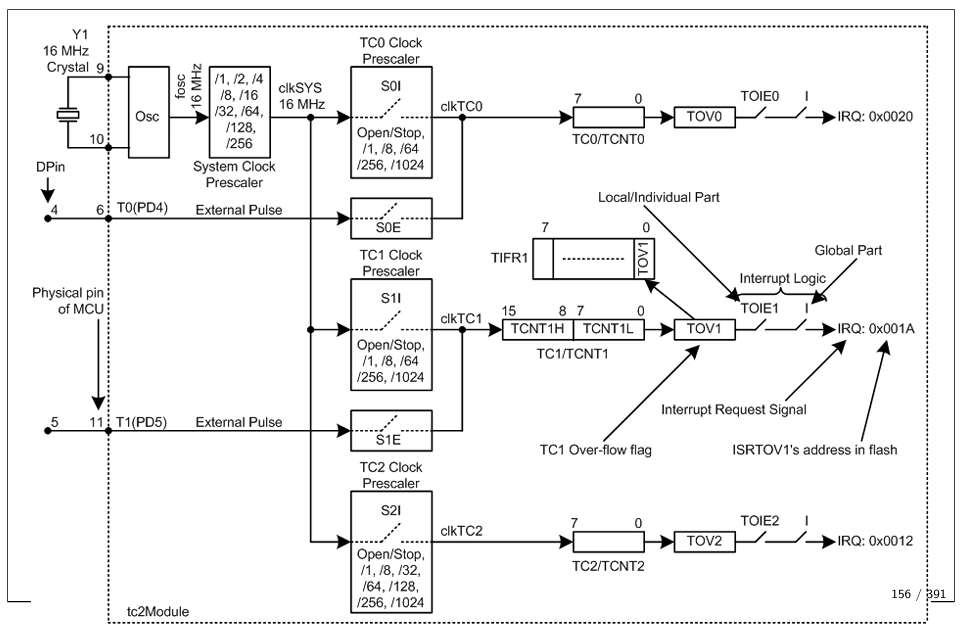
\includegraphics[width=0.75\textwidth]{Obrazky/Obrazky_DE2/fig_timer_structure.png}
    \caption{Štruktúra časovača ATmega328P. Hodinový signál (16 MHz) najprv prechádza predsdeličkou (prescaler), ktorá ho spomalí. Výsledný signál taktuje čítač TCNTn. Komparátor porovnáva TCNTn s hodnotou v OCRn. Výstupná jednotka autonómne generuje PWM na pine OCn.}
    \label{fig:timer_structure}
\end{figure}

\textbf{Preddelička (Prescaler):} hodinový signál 16 MHz je príliš rýchly pre väčšinu aplikácií. Preddelička ho vydelí pevnou hodnotou ($N \in \{1, 8, 64, 256, 1024\}$) a tým spomalí čítanie. S prescalerom 1024 sa čítač inkrementuje len $16\,000\,000 / 1024 \approx 15\,625\times$ za sekundu.

\section{Pretečenie -- čo sa stane, keď čítač dočíta}

8-bitový čítač počíta 0, 1, 2, \ldots, 254, 255 a potom \textbf{pretečie} späť na 0. Toto pretečenie (overflow) je dôležitá udalosť:
\begin{itemize}
    \item Nastaví sa príznak \textbf{TOVn} (Timer Overflow Flag)
    \item Ak je povolené prerušenie, CPU zavolá obslužnú rutinu
\end{itemize}

\begin{figure}[H]
    \centering
    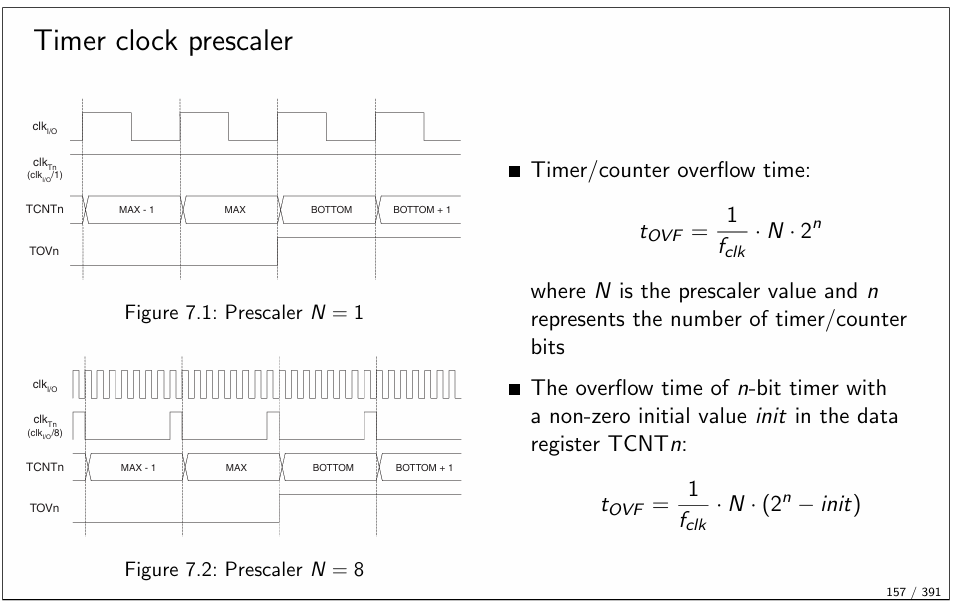
\includegraphics[width=0.80\textwidth]{Obrazky/Obrazky_DE2/fig_timer_overflow.png}
    \caption{Pretečenie čítača pri dvoch rôznych hodnotách prescaleru. Hore ($N=1$): čítač sa inkrementuje každý hodinový takt a preteká rýchlo. Dole ($N=8$): čítač sa inkrementuje len každý 8. takt -- preteká 8× pomalšie. Príznak TOVn sa nastaví vždy pri pretečení.}
    \label{fig:timer_overflow}
\end{figure}

\textbf{Ako vypočítať dobu pretečenia?} Čas pretečenia = (počet krokov čítača) × (perióda jedného kroku) = $2^n \times \dfrac{N}{f_{clk}}$.

Pre ATmega (16 MHz), Timer0 (8-bit), prescaler 64: $256 \times \dfrac{64}{16\,000\,000} = 1\,\text{ms}$ približne. Každú milisekundu pretečie.

\textbf{Inicializácia TCNTn:} ak nechceme čakať na plné pretečenie, načítame do TCNTn nenulovú hodnotu -- čítač potom začne od nej a pretečie skôr. Napr. načítame 206: čítač počíta 206, 207, \ldots, 255, potom pretečie. To je len 50 krokov namiesto 256.

\section{Komparácia -- presné časové intervaly}

Namiesto čakania na pretečenie môžeme nastaviť \textbf{porovnávaciu hodnotu v registri OCRn}. Komparátor neustále porovnáva TCNTn s OCRn. Pri zhode nastane \textbf{Compare Match}:
\begin{itemize}
    \item Nastaví sa príznak OCFn
    \item Môže sa vyvolať prerušenie
    \item Môže sa automaticky prepnúť výstupný pin (OCn)
\end{itemize}

\begin{figure}[H]
    \centering
    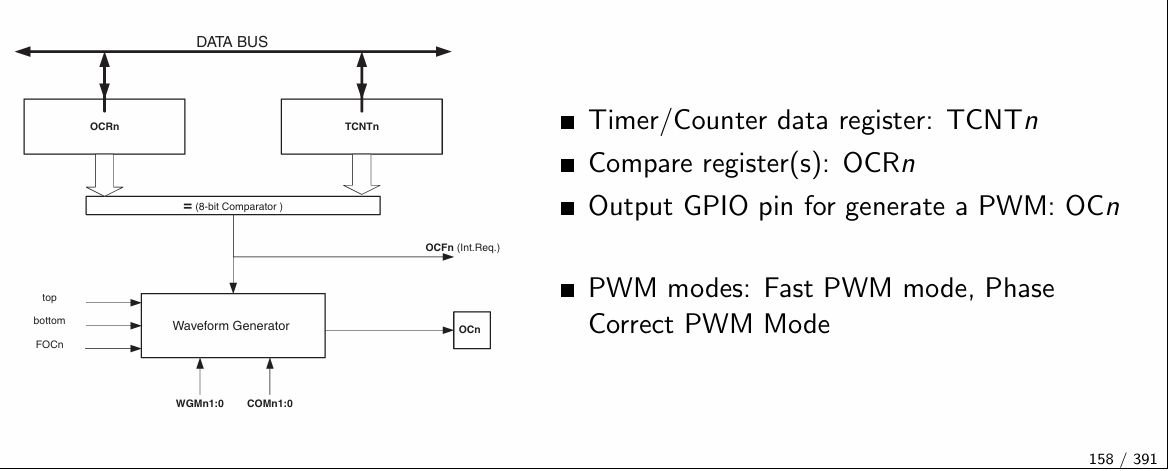
\includegraphics[width=0.65\textwidth]{Obrazky/Obrazky_DE2/fig_timer_compare.png}
    \caption{Blokové schéma komparačnej jednotky. Komparátor porovnáva TCNTn s OCRn. Pri zhode signalizuje zhodu (OCFn = prerušenie) a odovzdá pokyn Waveform Generatoru, ktorý podľa nastaveného módu (Fast PWM, Phase Correct PWM alebo CTC) riadi výstupný pin OCn.}
    \label{fig:timer_compare}
\end{figure}

\textbf{CTC mód (Clear Timer on Compare Match):} pri zhode TCNTn = OCRnA sa čítač \textbf{automaticky vynuluje} a začne znova od 0. Výsledkom je presne periodické prerušenie s nastaviteľnou periódou.

Praktické využitie: funkcia \texttt{millis()} v Arduine. Timer1 je nastavený v CTC móde tak, aby generoval prerušenie každú milisekundu. V obsluhe prerušenia sa inkrementuje globálna premenná -- a \texttt{millis()} ju len vráti.

\section{PWM -- riadenie výkonu digitálnym signálom}

\textbf{PWM (Pulse Width Modulation)} rieši problém: ako riadiť analógovú veličinu (jas LED, rýchlosť motora) digitálnym signálom (len 0 alebo 1)?

Riešenie: \textbf{signál rýchlo prepína medzi 0 a 1}. Ak je po väčšiu časť času v stave 1, priemerné napätie je vysoké -- LED svieti jasne. Ak je po väčšiu časť času v stave 0, priemerné napätie je nízke -- LED svieti slabo. Oko ani motor to nedokážu rozlíšiť.

\textbf{Strida (Duty Cycle):} pomer doby zapnutia k celkovej perióde, v percentách. 25\% strida = štvrtina periódy zapnutá. $V_{avg} = DC \cdot V_{CC}$.

\subsection{Fast PWM mód}

Čítač počíta \textbf{jedným smerom} -- od 0 nahor až do MAX, potom skočí späť na 0.

\begin{figure}[H]
    \centering
    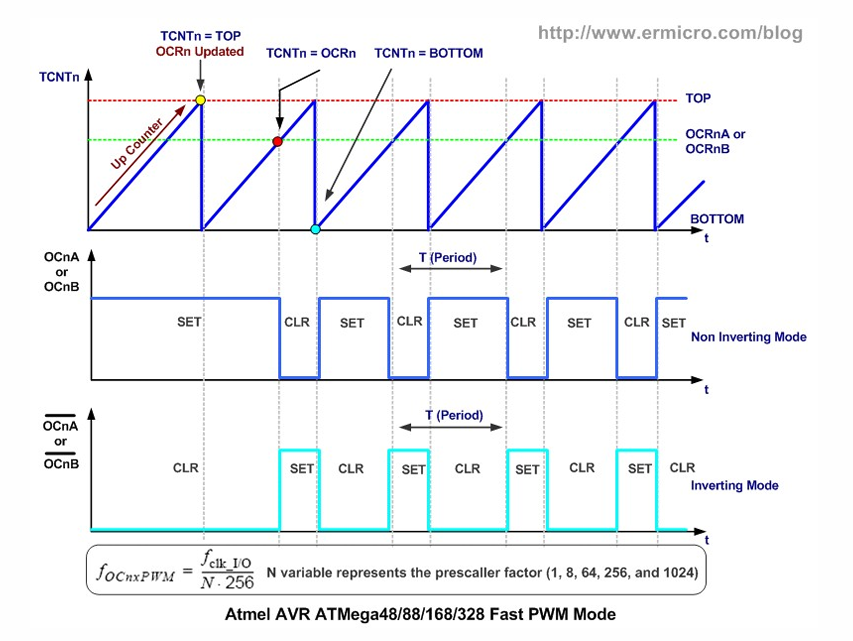
\includegraphics[width=0.75\textwidth]{Obrazky/Obrazky_DE2/fig_fast_pwm.png}
    \caption{Fast PWM mód. TCNTn (tučná píla) rastie od 0 do MAX, potom skočí späť. Výstup OCn sa nastaví na 1 vždy pri pretečení (TCNTn = 0) a vynuluje sa pri zhode s OCRn. Čím vyššie OCRn, tým dlhšia je časť s vysokou úrovňou -- tým vyššia strida. Frekvencia PWM závisí od hodinového kmitočtu, prescaleru a rozlíšenia čítača.}
    \label{fig:fast_pwm}
\end{figure}

Strida sa riadi hodnotou OCRn: OCRn = 0 znamená 0\% (stále nízka), OCRn = MAX znamená 100\% (stále vysoká). Frekvencia PWM je daná rýchlosťou čítania.

\subsection{Phase Correct PWM mód}

Čítač počíta \textbf{oboma smermi} -- nahor od 0 do MAX, potom nadol späť na 0.

\begin{figure}[H]
    \centering
    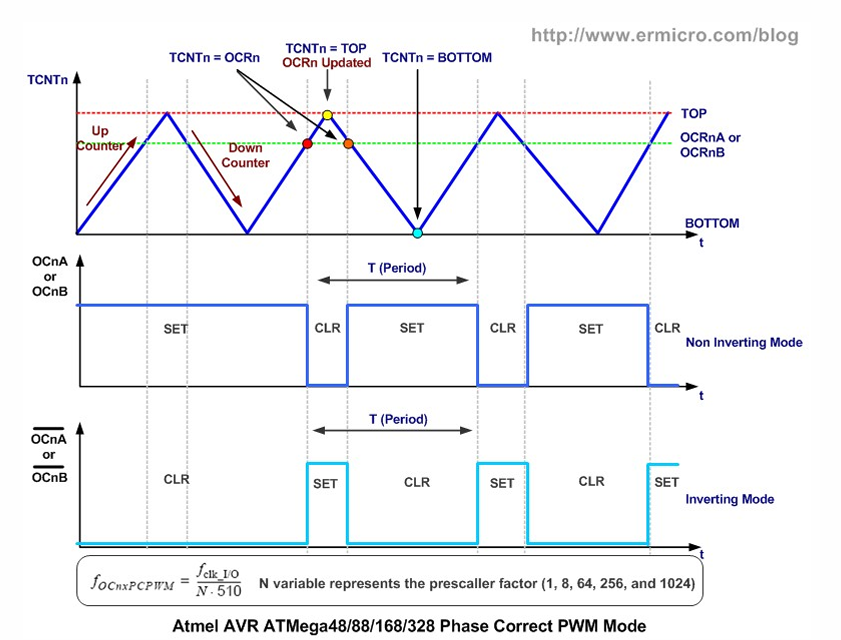
\includegraphics[width=0.75\textwidth]{Obrazky/Obrazky_DE2/fig_phase_correct_pwm.png}
    \caption{Phase Correct PWM mód. TCNTn tvorí trojuholníkový priebeh -- rastie a klesá. Výstup sa nuluje pri zhode na ceste nahor a nastavuje pri zhode na ceste nadol. Výsledný PWM pulz je symetrický okolo stredu periódy -- to je výhodné pre riadenie motorov.}
    \label{fig:phase_correct_pwm}
\end{figure}

\textbf{Prečo Phase Correct PWM pre motory?} Symetrický pulz spôsobuje menšie elektromagnetické rušenie. Navyše je fáza PWM na oboch kanáloch toho istého časovača vždy rovnaká -- to je dôležité pre H-mosty (riadenie smeru a rýchlosti motora).

\begin{center}
\begin{tabular}{lll}
\toprule
\textbf{Vlastnosť} & \textbf{Fast PWM} & \textbf{Phase Correct PWM} \\
\midrule
Smer čítania    & Jednosmerný (nahor)   & Obojsmerný (nahor/nadol) \\
Frekvencia      & Vyššia                & Približne polovičná \\
Symetria pulzu  & Nesymetrický          & Symetrický \\
Rušivosť (EMI)  & Vyššia                & Nižšia \\
Použitie        & LED, stmievanie, DAC  & Motory, servá \\
\bottomrule
\end{tabular}
\end{center}

%%%%%%%%%%%%%%%%%%%%%%%%%%%%%%%%%%%%%%%%%%%%%%%%%%%
\chapter{Sériová komunikácia UART a I2C}
%%%%%%%%%%%%%%%%%%%%%%%%%%%%%%%%%%%%%%%%%%%%%%%%%%%

\section{Prečo sériová komunikácia?}

Mikrokontroléry potrebujú komunikovať so senzormi, displejmi, GPS modulmi, Bluetooth, inými mikrokontrolérmi. Paralelná zbernica (8 vodičov pre 8 bitov) by bola drahá a nepraktická. \textbf{Sériová komunikácia} posiela bity jeden po druhom po jednom alebo dvoch vodičoch.

Kľúčové otázky každej sériovej komunikácie:
\begin{itemize}
    \item \textbf{Ako pozná prijímač, kde začína a končí jedno číslo (bajt)?} -- rámcovanie
    \item \textbf{Ako sa synchronizujú rýchlosti vysielača a prijímača?} -- synchronizácia
    \item \textbf{Ako sa na jednej zbernici rozlišujú rôzne zariadenia?} -- adresovanie
\end{itemize}

\section{UART -- najjednoduchšia sériová komunikácia}

UART (Universal Asynchronous Receiver/Transmitter) je najstarší a najjednoduchší sériový protokol. Prepája \textbf{presne dve zariadenia} dvoma vodičmi: TX (vysielanie) a RX (príjem).

\textbf{Asynchrónny} znamená: \textbf{žiadny zdieľaný hodinový signál}. Obe strany si musia dohodnúť rýchlosť (baud rate) vopred a každá si tiká vlastnými hodinami.

\subsection{Ako vyzerá UART rámec}

\begin{figure}[H]
    \centering
    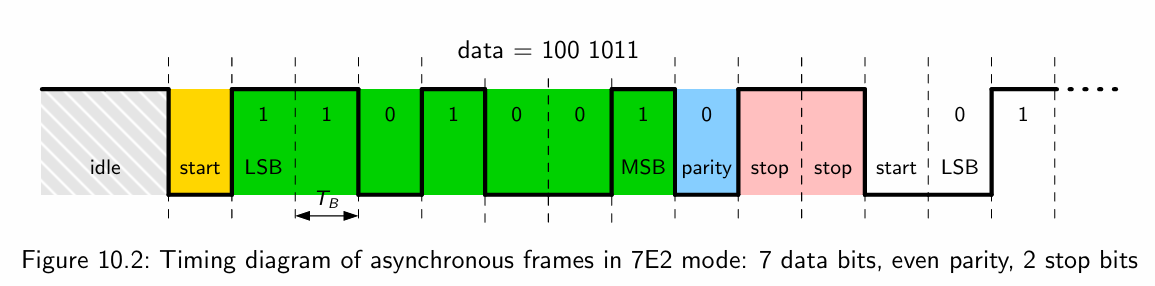
\includegraphics[width=0.85\textwidth]{Obrazky/Obrazky_DE2/fig_uart_frame.png}
    \caption{Časový diagram UART rámca (konfigurácia 7E2 pre prenos znaku 'K'). Linka je normálne v stave log. 1 (idle). Start bit (log. 0) upozorní prijímač. Potom prídu dátové bity od LSB. Paritný bit slúži na detekciu chýb. Jeden alebo dva stop bity (log. 1) ukončia rámec.}
    \label{fig:uart_frame}
\end{figure}

Každý bajt sa pošle ako \textbf{rámec}:
\begin{enumerate}
    \item \textbf{Start bit} (vždy log. 0): upozorní prijímač, že prichádzajú dáta
    \item \textbf{Dátové bity} (5--9, typicky 8): vlastné dáta, od LSB po MSB
    \item \textbf{Paritný bit} (voliteľný): súčet jednotiek, na detekciu jednoduchej chyby
    \item \textbf{Stop bit(y)}: linka sa vráti na log. 1, prijímač vie, že rámec skončil
\end{enumerate}

Označenie konfigurácie: \textbf{8N1} (8 dátových, bez parity, 1 stop -- najčastejší), \textbf{7E2} (7 dát, párna parita, 2 stop).

\textbf{Ako sa prijímač synchronizuje bez hodín?} Detekuje zostupnú hranu start bitu a potom vzorkuje každý bit v strede jeho časového okna. Interné hodiny prijímača tikajú 16× rýchlejšie ako baud rate -- start bit sa vzorkuje po 8 taktoch (stred), každý nasledujúci bit po 16 taktoch.

\textbf{Typické baud rates:} 9600, 19200, 57600, 115200 Bd (bitov za sekundu). Musia byť zhodné na oboch stranách!

\textbf{Využitie kanála:} pri 8N1 je z 10 prenesených bitov 8 dátových -- \textbf{80\% efektívnosť}. Zvyšných 20\% sú start a stop bity (réžia).

\textbf{Chybové príznaky:}
\begin{itemize}
    \item \textbf{Framing Error:} stop bit nie je log. 1 -- zlá rýchlosť alebo rušenie
    \item \textbf{Parity Error:} parita nesedí -- prevrátený jeden bit
    \item \textbf{Overrun Error:} nové dáta prišli skôr, ako CPU čítalo predchádzajúce
\end{itemize}

\subsection{USART v ATmega328P}

ATmega328P má perifériu USART na pinoch PD0 (RxD) a PD1 (TxD). Baud rate sa nastavuje zápisom do registra UBRR -- ten hovorí, koľkými hodinovými taktmi trvá jeden bit.

\section{I2C -- zbernica pre viac zariadení}

I2C (Inter-Integrated Circuit, vyslovuje sa ``I squared C'') vyvinul Philips v roku 1982 na prepojenie obvodov na jednej doske. Oproti UART pridáva kľúčové schopnosti: \textbf{viac zariadení na dvoch vodičoch} a \textbf{adresovanie}.

Iba \textbf{dva vodiče}:
\begin{itemize}
    \item \textbf{SCL} (Serial Clock): hodinový signál -- generuje ho vždy Master
    \item \textbf{SDA} (Serial Data): obojsmerná dátová linka
\end{itemize}

Oba vodiče sú cez odpory pripojené k napájaniu (pull-up). Každé zariadenie môže linku len \textbf{stiahnuť nadol} (open-drain) -- nikto linku aktívne nedvíha. Tým sa zabráni skratu pri kolízii.

Typické rýchlosti: 100 kHz (standard), 400 kHz (fast), 1 MHz (fast-plus).

\subsection{Ako I2C komunikácia prebieha -- krok za krokom}

\begin{figure}[H]
    \centering
    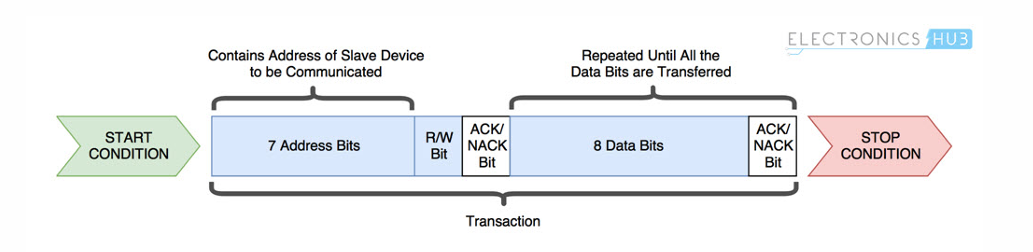
\includegraphics[width=0.85\textwidth]{Obrazky/Obrazky_DE2/fig_i2c_frame.png}
    \caption{Časový diagram I2C komunikácie. Dáta na SDA sú platné, keď SCL je vysoká. Start podmienka: SDA klesne, zatiaľ čo SCL je vysoká. Po Start podmienke Master pošle adresu Slave + bit R/W. Slave odpovie bitom ACK (stiahne SDA na 0). Potom sa prenášajú dátové bajty, každý potvrdený ACK. Stop podmienka: SDA stúpne pri vysokom SCL.}
    \label{fig:i2c_frame}
\end{figure}

\textbf{Celá sekvencia čítania z I2C senzora:}
\begin{enumerate}
    \item Master generuje \textbf{Start podmienku}: SDA klesne pri vysokom SCL -- všetky zariadenia to zaznamenajú
    \item Master pošle \textbf{7-bitovú adresu} Slave + bit R/W (0 = zápis)
    \item Oslovený Slave odpovie \textbf{ACK} (stiahne SDA na 0 v 9. takte) -- ostatné Slave ignorujú
    \item Master pošle \textbf{adresu registra}, z ktorého chce čítať; Slave potvrdí ACK
    \item Master generuje \textbf{Repeated Start} (nový Start bez Stop) + adresu Slave + bit R/W = 1 (čítanie)
    \item Slave pošle dáta; Master potvrdí ACK po každom bajte
    \item Po poslednom bajte Master pošle \textbf{NACK} (nestiahne SDA) -- signál, že nechce viac dát
    \item Master generuje \textbf{Stop podmienku}: SDA stúpne pri vysokom SCL
\end{enumerate}

\textbf{Clock Stretching:} Slave môže zdržať komunikáciu tým, že drží SCL nízko -- dáva si čas na spracovanie (napr. čaká na dokončenie merania). Master počká, kým Slave SCL neuvoľní.

\textbf{Repeated Start:} namiesto Stop + Start možno použiť Repeated Start (len nový Start bez Stop). Master tak udrží kontrolu nad zbernicou a prepne zo zápisu na čítanie v jednej transakcii.

\subsection{Adresovanie -- viac zariadení na jednej zbernici}

Každé I2C zariadenie má \textbf{unikátnu 7-bitovú adresu} (0--127, ale 16 je rezervovaných -- max. 112 zariadení). Adresa je buď pevne daná výrobcom, alebo čiastočne konfigurovateľná pomocou pinov (typicky 2--3 bity). Napríklad čip PCF8574 má základnú adresu 0x20 a piny A0--A2 umožňujú až 8 rôznych adries.

\subsection{I2C v ATmega328P -- TWI}

ATmega328P implementuje I2C ako \textbf{TWI (Two Wire Interface)} na pinoch PC4 (SDA) a PC5 (SCL). Frekvencia SCL sa nastavuje zápisom do registra TWBR.

\textbf{Príklady I2C zariadení:}
\begin{itemize}
    \item \textbf{DHT12}: senzor teploty a vlhkosti, adresa 0x5C
    \item \textbf{DS3231}: RTC hodiny reálneho času, adresa 0x68
    \item \textbf{AT24C32}: EEPROM pamäť 32 kB, adresa 0x57
    \item \textbf{PCF8574}: I/O expandér (pridá 8 GPIO pinov), adresy 0x20--0x27
\end{itemize}

\section{UART vs. I2C -- kedy čo použiť?}

\begin{center}
\begin{tabular}{lll}
\toprule
\textbf{Vlastnosť}    & \textbf{UART}                     & \textbf{I2C} \\
\midrule
Počet vodičov         & 2 (TX, RX)                        & 2 (SCL, SDA) \\
Počet zariadení       & 2 (point-to-point)                & Až 112 na jednej zbernici \\
Synchronizácia        & Asynchrónna (baud rate)           & Synchrónna (zdieľané hodiny) \\
Adresovanie           & Nie je -- priame spojenie         & 7-bitová adresa každého zariadenia \\
Duplex                & Full-duplex (súčasne oba smery)   & Half-duplex (striedavo) \\
Rýchlosť              & Až 115200 Bd (štd.)               & Až 400 kHz (fast mode) \\
Protokol              & Jednoduchý (len rámce)            & Zložitejší (Start/Stop/ACK) \\
Typické použitie      & Ladenie, GPS, Bluetooth, modem    & Senzory, EEPROM, RTC, displeje \\
\bottomrule
\end{tabular}
\end{center}

\textbf{UART volíme}, ak prepájame dve zariadenia, potrebujeme full-duplex alebo pracujeme s modulom, ktorý UART podporuje (GPS, Bluetooth modul, PC).

\textbf{I2C volíme}, ak pripájame viac senzorov alebo periférií k jednému mikrokontroléru a chceme šetriť piny (stačia vždy len 2 vodiče bez ohľadu na počet zariadení).